\documentclass[11pt]{amsart}
\usepackage{geometry} % see geometry.pdf on how to lay out the page. There's lots.
\geometry{a4paper} % or letter or a5paper or ... etc
% \geometry{landscape} % rotated page geometry
\usepackage{amsmath}
\usepackage{graphicx}
\usepackage{breqn}
\usepackage{amsthm, amssymb, amsmath, centernot}
\usepackage{slashed}
\newcommand{\notimplies}{%
  \mathrel{{\ooalign{\hidewidth$\not\phantom{=}$\hidewidth\cr$\implies$}}}}
 
\renewcommand\qedsymbol{$\square$}
\newcommand{\cont}{$\boxtimes$}
\newcommand{\divides}{\mid}
\newcommand{\ndivides}{\centernot \mid}
\newcommand{\Z}{\mathbb{Z}}
\newcommand{\N}{\mathbb{N}}
\newcommand{\C}{\mathbb{C}}
\newcommand{\Zplus}{\mathbb{Z}^{+}}
\newcommand{\Primes}{\mathbb{P}}
\newcommand{\ball}[2]{B_{#1} \! \left(#2 \right)}
\newcommand{\Q}{\mathbb{Q}}
\newcommand{\R}{\mathbb{R}}
\newcommand{\Rplus}{\mathbb{R}^+}
\newcommand{\invI}[2]{#1^{-1} \left( #2 \right)}
\newcommand{\End}[1]{\text{End}\left( A \right)}
\newcommand{\legsym}[2]{\left(\frac{#1}{#2} \right)}
\renewcommand{\mod}[3]{\: #1 \equiv #2 \: \mathrm{mod} \: #3 \:}
\newcommand{\nmod}[3]{\: #1 \centernot \equiv #2 \: mod \: #3 \:}
\newcommand{\ndiv}{\hspace{-4pt}\not \divides \hspace{2pt}}
\newcommand{\finfield}[1]{\mathbb{F}_{#1}}
\newcommand{\finunits}[1]{\mathbb{F}_{#1}^{\times}}
\newcommand{\ord}[1]{\mathrm{ord}\! \left(#1 \right)}
\newcommand{\quadfield}[1]{\Q \small(\sqrt{#1} \small)}
\newcommand{\vspan}[1]{\mathrm{span}\! \left\{#1 \right\}}
\newcommand{\galgroup}[1]{Gal \small(#1 \small)}
\newcommand{\bra}[1]{\left| #1 \right>}
\newcommand{\Oa}{O_\alpha}
\newcommand{\Od}{O_\alpha^{\dagger}}
\newcommand{\Oap}{O_{\alpha '}}
\newcommand{\Odp}{O_{\alpha '}^{\dagger}}
\renewcommand{\Im}[1]{\mathrm{Im} \: #1}
\newcommand{\ket}[1]{\left| #1 \right>}
\renewcommand{\bra}[1]{\left< #1 \right|}
\newcommand{\inner}[2]{\left< #1 | #2 \right>}
\newcommand{\expect}[2]{\left< #1 \right| #2 \left| #1 \right>}
\renewcommand{\d}[1]{ \mathrm{d}#1 \:}
\newcommand{\dn}[2]{ \mathrm{d}^{#1} #2 \:}
\newcommand{\deriv}[2]{\frac{\d{#1}}{\d{#2}}}
\newcommand{\pderiv}[2]{\frac{\partial{#1}}{\partial{#2}}}
\newcommand{\parsq}[2]{\frac{\partial^2{#1}}{\partial{#2}^2}}
\newcommand{\topo}{\mathcal{T}}
\newcommand{\base}{\mathcal{B}}
\renewcommand{\bf}[1]{\mathbf{#1}}
\renewcommand{\a}{\hat{a}}
\newcommand{\adag}{\hat{a}^\dagger}
\renewcommand{\b}{\hat{b}}
\newcommand{\bdag}{\hat{b}^\dagger}
\renewcommand{\c}{\hat{c}}
\newcommand{\cdag}{\hat{c}^\dagger}
\newcommand{\hamilt}{\hat{H}}
\renewcommand{\L}{\hat{L}}
\newcommand{\Lz}{\hat{L}_z}
\newcommand{\Lsquared}{\hat{L}^2}
\renewcommand{\S}{\hat{S}}
\renewcommand{\empty}{\varnothing}
\newcommand{\J}{\hat{J}}
\newcommand{\lagrange}{\mathcal{L}}
\newcommand{\dfourx}{\mathrm{d}^4x}
\newcommand{\meson}{\phi}
\newcommand{\dpsi}{\psi^\dagger}
\newcommand{\ipic}{\mathrm{int}}
\newcommand{\parity}{\mathbf{P}}
\newcommand{\conj}{\mathbf{C}}
\newcommand{\tr}[1]{\mathrm{Tr} \left( #1 \right)}

\renewcommand{\theenumi}{(\alph{enumi})}

\newcommand{\atitle}[1]{\title{% 
	\large \textbf{Physics GR6047 Quantum Field Theory I
	\\ Assignment \# #1} \vspace{-2ex}}
\author{Benjamin Church }
\maketitle}

 
\newtheorem{theorem}{Theorem}[section]
\newtheorem{lemma}[theorem]{Lemma}
\newtheorem{proposition}[theorem]{Proposition}
\newtheorem{corollary}[theorem]{Corollary}
\newtheorem{remark}[theorem]{Remark}
 




\setcounter{MaxMatrixCols}{10}

\flushbottom
\chardef\atcode=\catcode`\@
\makeatletter
\@addtoreset{figure}{section}
\@addtoreset{table}{section}
\renewcommand{\figurename}{Figure}
\renewcommand{\tablename}{Table}
\setcounter{topnumber}{3}               % orig: 2
\setcounter{totalnumber}{4}             % orig: 3
\renewcommand{\textfraction}{0}         
\renewcommand{\bottomfraction}{0.65}    
\renewcommand{\topfraction}{0.75}       
\renewcommand{\floatpagefraction}{0.75} 
\catcode`\@=\atcode 
\newcommand{\grad}{$^\circ$}
\newcommand{\gradm}{^\circ}
\newcommand{\bqn}{ \begin{eqnarray} }
\newcommand{\eqn}{ \end{eqnarray} }
\newcommand{\beq}{ \begin{equation} }
\newcommand{\eeq}{ \end{equation} }
\setlength{\baselineskip}{2.1ex}
\renewcommand{\baselinestretch}{1.06}
\setlength{\parskip}{1.5ex plus 0.8ex minus 0.6ex}
\setlength{\evensidemargin}{0.3cm}
\setlength{\oddsidemargin}{0.2cm}
\setlength{\topmargin}{-1cm}
\setlength{\textwidth}{16.5cm}
\setlength{\textheight}{26cm}
\newcommand{\mat}[1]{\mbox{$\underline{\underline{#1}}$}}
\newcommand{\etal}{\mbox{\sl et al.}}
\renewcommand{\refname}{}
\newcommand{\vol}[1]{{\bf{#1}}}
\newcommand{\dg}{$^\circ\;$}
\def\D{\displaystyle}
\newcommand{\lapprox}{\ensuremath{<\atop{\mbox{\raisebox{0.5ex}{$\sim$}}}}}
\parindent 0cm
\usepackage{gensymb}

% See the ``Article customise'' template for come common customisations

\title{Physics UN2801 Fall 2018 Problem Set 1}
\author{Benjamin Church}
%\date{Sept 12} % delete this line to display the current date

%%% BEGIN DOCUMENT
\begin{document}


\maketitle

\section{Problem 1. Approximations}

a.) A Taylor Expansion is a way of representing a function as an infinite sum of terms and is a way to represent functions in simpler forms that are easier to use mathematically. This problem asks you to take expansion of $\tan{\theta}$. The general form of a Taylor Expansion around a particular value a is, 
\begin{eqnarray*}
f(x) &=& f(a)+\frac{f^{'}(a)}{1!} (x-a)+\frac{f^{''}(a)}{2!}(x-a)^{2}+\frac{f^{'''}(a)}{3!}(x-a)^{3} + \cdots = \sum^{\infty}_{n=0} \frac{f^{(n)}}{n!}(x-a)^{n} 
\\
n! &=& n(n-1)(n-2)(n-3)(n-4) \cdots 
\end{eqnarray*} 
In the case the value to expand around is $\theta=0$, which means in the equation above $a=0$. Start by taking the derivatives of $\tan{\theta}$ with respect to $\theta$. $tan(0)=0$ so the first 3 nonzero terms are the ones that contain the first 3 derivatives. \\
\begin{eqnarray*}
\frac{d\tan{\theta}}{d\theta} &=& \sec^{2}(\theta) 
\\
\frac{d^{2}\tan{\theta}}{d\theta^{2}} &=& 2\sec(\theta)\frac{d \sec(\theta)}{d\theta} = 2\sec(\theta)\sec(\theta)\tan{\theta} = 2\sec^{2}(\theta)\tan{\theta} 
\\
\frac{d^{3}\tan{\theta}}{d\theta^{3}} &=& 2(2\sec^{2}(\theta)\tan{\theta}\tan{\theta} + \sec^{2}(\theta)sec^{2}(\theta)) = 2\sec^{2}(\theta)(2\tan^{2}(\theta) + \sec^{2}(\theta)) 
\end{eqnarray*} 
Now put this into the expansion: \\
\begin{eqnarray*} 
\tan{\theta} &\approx& tan(0) + \frac{sec^{2}(0)}{1!}(\theta-0) + \frac{2sec^{2}(0)tan(0)}{2!}(\theta-0)^{2} + \frac{2sec^{2}(0)(2tan^{2}(0) + sec^{2}(0))}{3!}(\theta-0)^{3} \nonumber \\
\tan{\theta} &\approx& 0 + \theta + 0 + 2\cdot \frac{0 + 1}{3 \cdot 2 \cdot 1}\theta^{3} = \theta + (2/6)\theta^{3}  \\
\tan{\theta} &\approx& \theta + \frac{\theta^{3}}{3}  
\end{eqnarray*}  \\
To see a quicker was of doing this look at the end of part b of this problem. Then the problem states that $\theta<<1$  so that $\tan{\theta}$ can be approximated by the first term in the expansion. This is a very important concept to remember because this is often used to approximate solutions to physics problems and you will do this often in this course and in the future. Remember that functions can be approximated through the Taylor Expansion and then if the arguments are small they can be approximated further by dropping terms. This approximation is called the small-angle approximation and can be used on other trigonometric functions also. This then makes solving problems a lot easier. \\
\begin{eqnarray*}
\tan{\theta} &\approx& \theta 
\end{eqnarray*} \\
The problem goes on to discuss the relative error of the expansion. This tells you how accurate the approximation you made actually is for different values of $\theta$. This relative error is found by taking the ratio of the second non-zero term in the expansion to the first: \\
\begin{eqnarray*} 
err_{rel} &\approx& \frac{\theta^{3}/3}{\theta}  = \theta^{2}/3 
\end{eqnarray*} \\
Then you can use different values of $\theta$ to figure out how accurate the approximation is. The problem asks you to work backward though and find the values of $\theta$ that give you certain errors. Keep in mind that when you do the Taylor Expansion in $\theta$, the $\theta$ is in radians not degrees. Thus in order to complete the problem the angle has to be converted to degrees to get both like the problem asks for. The different errors given are 10, 1, and 25 percent. \\
\begin{eqnarray*}
err_{rel} &\approx& \theta^{2}/3  \\
\theta &\approx& 3\sqrt{err_{rel}}  \\
\theta &\approx& 3\sqrt{0.1} = 0.94868 \mbox{ rad}  \\
\theta &\approx& (0.94868)\frac{180}{\pi} = 54.356\degree  \\
\theta &\approx& 3\sqrt{0.01} = 0.3 \mbox{ rad}  \\
\theta &\approx& (0.3)\frac{180}{\pi} = 17.189\degree  \\
\theta &\approx& 3\sqrt{0.25} = 1.5 \mbox{ rad}  \\
\theta &\approx& (1.5)\frac{180}{\pi} = 85.944\degree  
\end{eqnarray*} \\ 
b.) This part is about the binomial approximation, which is another very important and useful approximation for solving physics problems. The formula is as follows, where $\delta<<1$ and a is any power (positive or negative): \\
\begin{eqnarray*}
(1+\delta)^{a} &\approx& 1 + a\delta 
\end{eqnarray*} \\
The problem asks for you to do this on the hypotenuse of a right triangle with sides d and L, where $d<<L$. The equation for this is as follows: \\
\begin{eqnarray*}
h &=& \sqrt{L^{2} + d^{2}} 
\end{eqnarray*}\\
The first step is to manipulate this equation to look like the general equation for the binomial expansion so the approximation can be directly applied. This means factoring out the $L^{2}$ to get a 1 as the first term and turning the square root into a power: \\  
\begin{eqnarray*} 
h &=& \sqrt{L^{2} \left(1 + \frac{d^{2}}{L^{2}} \right)} = L\left(1 + \frac{d^{2}}{L^{2}} \right)^{1/2} 
\end{eqnarray*} \\
Then apply the approximation where $\delta=\frac{d^{2}}{L^{2}}$ and $a=1/2$ to get: \\ 
\begin{eqnarray*}
h &\approx& L(1 + (1/2)\frac{d^{2}}{L^{2}}) = L + \frac{d^{2}}{2L} 
\end{eqnarray*}  \\
This technique could have helped simplify the work you had to do for part a. Instead of taking derivatives of tangent multiple times, you could have done this: \\ 
\begin{eqnarray*} 
\tan{\theta} &=& \frac{\sin{\theta}}{\cos{\theta}}  \\
\sin{\theta} &\approx& \sin(0) + \cos(0) x -(1/2)\sin(0) x^{2} - (1/6) \cos(0) x^{3} = x - x^{3}/6  \\
\cos{\theta} &\approx& \cos(0) - \sin(0) x -(1/2) \cos(0) x^{2} + (1/6) \sin(0)x^{3} = 1 - x^{2}/2
\\
\tan{\theta} &\approx& \frac{x - x^{3}/6}{1-x^{2}/2} = \left(x - x^{3}/6 \right)\left(1-x^{2}/2 \right)^{-1} \mbox{ (use binomial expansion)}  \\
\tan{\theta} &\approx& (x-\frac{x^{3}}{6})(1+\frac{x^{2}}{2}) = x+\frac{x^{3}}{2}-\frac{x^{3}}{6}-\frac{x^{5}}{12} \mbox{ (drop the last term because it is of higher order)}  \\
\tan{\theta} &\approx& x + x^{3}/3  
\end{eqnarray*} \\
This is the same answer we got for part a, with a lot less work. \\ \\ 
c.) Here the problem asks to show that the sum of two Taylor Expansions is the same as the Taylor Expansion of the sum. Suppose $f$ and $g$ have Taylor series,
\begin{eqnarray*} 
f(x) &=& f(a) + \frac{f^{'}(a)}{1!} (x-a) + \frac{f^{''}(a)}{2!}(x-a)^{2} + \frac{f^{'''}(a)}{3!}(x-a)^{3} + \cdots  
\\
g(x) &=& g(a) + \frac{g^{'}(a)}{1!} (x-a) + \frac{g^{''}(a)}{2!}(x-a)^{2} + \frac{g^{'''}(a)}{3!}(x-a)^{3} + \cdots  
\end{eqnarray*}
then the Taylor series of the sum is,
\[ f(x) + g(x) = f(a) + g(a) + \frac{(f+g)^{'}(a)}{1!} (x-a) + \frac{(f+g)^{''}(a)}{2!}(x-a)^{2} + \frac{(f+g)^{'''}(a)}{3!}(x-a)^{3} + \cdots \]
By the linearity of the derivative,
\[ (f + g)^{(n)}(a) = f^{(n)}(a) + f^{(n)}(a) \]
and therefore,
\begin{align*}
f(x) + g(x) & = f(a) + g(a) + \frac{(f+g)^{'}(a)}{1!} (x-a) + \frac{(f+g)^{''}(a)}{2!}(x-a)^{2} + \frac{(f+g)^{'''}(a)}{3!}(x-a)^{3} + \cdots
\\
& = f(a) + g(a) + \frac{f^{'}(a) + g^{'}(a)}{1!} (x-a) + \frac{f^{''}(a) + g^{''}(a)}{2!}(x-a)^{2} + \frac{f^{'''}(a) + g^{'''}(a)}{3!}(x-a)^{3} + \cdots
\\
& = f(a) + \frac{f^{'}(a)}{1!} (x-a) + \frac{f^{''}(a)}{2!}(x-a)^{2} + \frac{f^{'''}(a)}{3!}(x-a)^{3} + \cdots 
\\
& + g(a) + \frac{g^{'}(a)}{1!} (x-a) + \frac{g^{''}(a)}{2!}(x-a)^{2} + \frac{g^{'''}(a)}{3!}(x-a)^{3} + \cdots 
\end{align*} 
Thus we arrived at the form for the expansion of the two functions added together. The fact that the Taylor Expansions adds linearly really just follows from the linearity of the derivative but this is, none the less, an important tool for approximating larger, more complicated approximations.
\\\\
d.) This part asks you to make an expansion of a more complicated function to first order in $x/a$ where $x<<a$. It states that is can be done using either the Taylor Expansion explicitly or by doing the binomial expansion. I will show you both, starting with the Taylor Expansion. The first thing to notice is that this is 2 functions added together. Therefore, we can use the proof from part c of this problem set to do each function separately and then add them together at the end. We can compute the Taylor series or use the well-known series,
\[ \frac{1}{1 - x} = 1 + x + x^2 + \cdots \]
to compute,
\[ \frac{1}{a + x} = \frac{1}{a} \cdot \frac{1}{1 + a / x} = \frac{1}{a} \left(1 - (x / a) + \cdots \right) \]
and similary,
\[ \frac{1}{a - x} = \frac{1}{a} \cdot \frac{1}{1 + a / x} = \frac{1}{a} \left(1 + (x / a) + \cdots \right) \]
To first-order, the Taylor series is exactly the same as the Binomial approximation,
\[ 
\left(1 + a / x \right)^{-1} \approx 1 - a /x \]
Putting this together,
\begin{eqnarray*} 
\frac{1}{x + a} - \frac{1}{x - a} \approx \frac{1}{a} \left( 1 - a /x \right) - \frac{1}{a} \left( 1 + a /x \right) = - \frac{2 x}{a^2} 
\end{eqnarray*}

e.) This part asks you to take the binomial approximation of the same fractions, just added together and with an addition term. Use the results from part d for the binomial approximation and find the combination: \\ 
\begin{eqnarray*}
\frac{1}{a+x} + \frac{1}{a-x} - \frac{2}{a} &\approx& 1/a - x/a^{2} + 1/a + a/a^{2} -2/a = 2/a - 2/a = 0 
\end{eqnarray*} \\
Getting zero is a problem here because it means we have approximated away all the information in the function. If you use the result for the Taylor Expansion you also get the same issue since the results were the same. Thus, the solution is to take the expansion out to the next term. There is a formula for the binomial expansion out to the second term but since that may be a rather unused formula I will be using the next term from the expansion,
\begin{align*}
\frac{1}{a + x} & = \frac{1}{a} \cdot \frac{1}{1 + x/a} = \frac{1}{a} \left( 1 - (x / a) + (x / a)^2 + \cdots \right)
\\
\frac{1}{a - x} & = \frac{1}{a} \cdot \frac{1}{1 + x/a} = \frac{1}{a} \left( 1 + (x / a) + (x / a)^2 + \cdots \right)
\end{align*}
Thus, to second order in $x/a$ we get,
\[ \frac{1}{a+x} + \frac{1}{a-x} - \frac{2}{a} = \frac{2 x^2}{a^3} \]
Whenever you get zero from an approximation it only means the quantity is zero \textit{to the order of the approximation} that you made. This is not particularly helpful since you lost most of the information you were trying to get. Go to higher order approximations until you find something non-zero. The quantity you find if you stop going right when you find a non-zero value is called the leading-order approximation. 

\section{Problem 2. Oscillation Acceleration} 

This problem asks you to calculate the velocity and position for a time-dependent acceleration. 
\\ 
\[
a(t) = \left(\frac{eE_{0}}{m}\right) \cos(\omega{}t) = a_{0} \cos(\omega{}t) 
\]
where we have set,
\[ a_0 = \frac{ e E_0 }{m} \]
It is a good trick in physics problems that involve a lot of constants or just a lot of terms to make substitutions, like the book did for $a_{0}$, in order to simplify the math. \\ \\
The next step is to integrate this and find the velocity by doing $a=dv/dt$ and grouping the velocity and t terms on opposite sides of the equations like Brian did in lecture. Don't forget the dummy variables under the integral sign. The initial velocity is $v_{0}$ and $t_{0}=0$.
\begin{align*}
v(t) - v_0 = \int_{t_0}^t \deriv{v}{t} = \int_0^t a_0 \cos{(\omega t')} \d{t'} = a_0 \left[ \frac{1}{\omega} \sin{(\omega t)} \right]^t_0 = \frac{a_0}{\omega} \sin{(\omega t)}
\end{align*}
Now integrate again to get the position where $v(t)=dx/dt$ and the initial position $x_{0}$.
\begin{align*}
x(t) - x_0 = \int_{t_0}^t \deriv{x}{t} = \int_0^t \left( \frac{a_0}{\omega} \sin{(\omega t)} + v_0 \right) \d{t'} = v_0 t + \frac{a_0}{\omega^2} \left[ 1 - \cos{(\omega t)} \right] 
\end{align*}
The problem then states that $v_{0}=x_{0}=0$ so,
\begin{eqnarray*}
v(t) &=& - \frac{a_{0}}{\omega} \sin(\omega{}t) 
\\
x(t) &=& \frac{a_{0}}{\omega^{2}}(1 - \cos(\omega{}t)) 
\end{eqnarray*} \\
The problem then asks you to compare the result to those in the book, which are: \\ 
\begin{eqnarray*} 
v(t) &=& -\frac{a_{0}}{\omega}(\cos(\omega{}t) - 1) \\
x(t) &=& \frac{a_{0}}{\omega}t - \frac{a_{0}}{\omega^{2}} \sin(\omega{}t) 
\end{eqnarray*} \\
Look at the limits in the velocity equation. Our equation can have velocities anywhere from $v=-a_{0}/\omega$ to $v=a_{0}/\omega$. The book equation can have  velocities anywhere from $v=0$ to $v=2a_{0}/\omega$. Thus, the book equation for velocity is the kind of like the ``square'' of our equation because the have the same zeros but the book equation remains positive. Use the half-angle formula to prove this: \\
\begin{eqnarray*}
\sin^{2}(x) &=& (1/2)(1 - \cos(2x)) 
\\
\sin^{2}(x/2) &=& (1/2)(1 - \cos(2x)) 
\\ 
v(t) &=& \frac{a_{0}}{\omega}(1 - \cos(\omega{}t)) = \frac{2a_{0}}{\omega} \sin^{2}(\omega{}t) 
\\ 
\end{eqnarray*} \\
Thus, the are both oscillating velocities but one remains positive with a higher amplitude while the other oscillates between  positive and negative values. \\ \\
Do the same thing for the position equation. Our equation ranges from $x=0$ to $x=\frac{2a_{0}}{\omega^{2}}$. The book equation ranges from $x=\frac{a_{0}}{\omega^{2}}(\pi/2\omega-1)$ and $x=\frac{a_{0}}{\omega^{2}}(\pi/2\omega+1)$. This isn't exactly the same because of the first term in the book equation, but you can rearrange our equation using the half-angle formula again.\\ 
\begin{eqnarray*} 
x(t) &=& \frac{2a_{0}}{\omega^{2}} \sin^{2}(\omega{}t) 
\end{eqnarray*} \\
Thus for the position our equation is always positive and the book equation oscillates between positive and negative values with an offset. \\ 

\section{Problem 3. Integrating $\dot{x}$ when expressed as a function of $x$ instead of $t$.} 

Brian mentions a transcendental equation in his description of this problem. A transcendental equation is an equation that can not be solved analytically but can be solved graphically, numerically, or by making approximations on the functions to be simpler functions that can be solved. An example is here, which can not be solved directly for x: \\ 
\begin{eqnarray*}
e^{x} &=& x^{2} - \ln(x) 
\end{eqnarray*}
a.) A very important common equation to solve in physics: \\ 
\begin{eqnarray*} 
\frac{dx}{dt} &=& -\frac{x}{\tau} \\
x(t_{0}) &=& x_{0} 
\end{eqnarray*}  \\
The first step is to collect all the terms that involve x on one side and the ones that involve t on the other so you can integrate both sides with respect to one variable as Brian did in his second equation in the problem: \\ 
\begin{eqnarray*} 
\frac{dx}{x} &=& -\frac{dt}{\tau} 
\end{eqnarray*} \\
Then integrate both sides and don't forget to change the variables to a dummy variable and put in the limits as Brian does in his 3rd equation in the problem. \\ 
\begin{eqnarray*} 
\int^{x}_{x_{0}}\frac{1}{x'}\,dx' &=& \int^{t}_{t_{0}}-\frac{1}{\tau}\,dt' \\
\ln(x')|^{x}_{x_{0}} &=& -\frac{t'}{\tau}|^{t}_{t_{0}} \\
\ln(x) - \ln(x_{0}) &=& -(t - t_{0})/\tau \\
\ln(x/x_{0}) &=& -(t - t_{0})/\tau 
\\
x/x_{0} &=& e^{-\frac{t-t_{0}}{\tau}} 
\\
x(t) &=& x_{0}e^{-\frac{t-t_{0}}{\tau}} 
\end{eqnarray*}
This is an important functional form where the distance is exponentially decreasing and ``time constant'' is $\tau$.  The units in equation (1) are $[m]/[s] = [m]/[s]$ so they work out. In the final solution the units in the exponential are $[s]/[s]$ because the time constant has dimensions of seconds. Then outside of the exponential the units are $[m]=[m]$. It is important to remember unit analysis when solving physics problems because it can really help you figure out if your solution makes sense and also can lead you to where you went wrong. It also helps you develop a better understanding of what your solutions actually means and gives you a better physical intuition beyond the mathematics. \\ \\
b. The problem asks what happens if there is a plus sign instead of a minus sign in equation 1. The only thing that would change is that it would be a positively increasing exponential: \\ 
\begin{eqnarray*} 
\frac{dx}{dt} &=& \frac{x}{\tau} \\
x(t_{0}) &=& x_{0} \\
\int^{x}_{x_{0}}\frac{1}{x'}\,dx' &=& \int^{t}_{t_{0}}\frac{1}{\tau}\,dt' \\
\ln(x')|^{x}_{x_{0}} &=&\frac{t'}{\tau}|^{t}_{t_{0}} \\
\ln(x) - \ln(x_{0}) &=& (t - t_{0})/\tau \\
\ln(x/x_{0}) &=& (t - t_{0})/\tau \\
x/x_{0} &=& e^{\frac{t-t_{0}}{\tau}} \\
x(t) &=& x_{0}e^{\frac{t-t_{0}}{\tau}} 
\end{eqnarray*} \\
For large arbitrary x this function would not make physical sense because as $t \to \infty$ we have $x(t) \to \infty$ in such a way that the acceleration, velocity, and energy all blow up and become infinite. Such a system would produce an infinite amount of energy. 
\\  \\
c.) Solve a more complicated, but frequently encountered equation in physics. \\ 
\begin{eqnarray*} 
\frac{dx}{dt} &=& x_{0}\omega{}\sqrt{1 - \frac{x^{2}}{x_{0}^{2}}} \\
\frac{dx}{\sqrt{1 - \frac{x^{2}}{x_{0}^{2}}}} &=& x_{0}\omega{}dt \mbox{ (group x and t terms)} \\
\int^{x}_{x_{0}}\frac{1}{\sqrt{1 - \frac{(x')^{2}}{x_{0}^{2}}}}\,dx' &=& \int^{t}_{t_{0}}x_{0}\omega\,dt' = x_{0}\omega{}(t - t_{0}) 
\end{eqnarray*} \\
Lets evaluate the left hand integral separately. This will involve the trigonometric substitution $x' = x_0 \sin{\theta}$.
\begin{eqnarray*} 
\int^{x}_{x_0} 
\frac{1}{\sqrt{1 - \frac{(x')^{2}}{x_{0}^{2}}}}
\, \d{x'} 
&=& \int^{\sin^{-1}(x/x_0)}_{\pi/2} 
\frac{x_{0}\cos{\theta}}{\sqrt{1 - \sin^{2}(\theta)}} \, \d{\theta}  
\mbox{ (plug in the new trig substitution)} 
\\
&=& \int^{\sin^{-1}(x/x_0)}_{\pi/2} 
\frac{x_{0}\cos{\theta}}{\sqrt{\cos^{2}(\theta)}}\, \d{\theta}
\\
&=& \int^{\sin^{-1}(x/x_0)}_{\pi/2} 
\frac{x_{0}\cos{\theta}}{\cos{\theta}}\,d\theta 
\\
&=& \int^{\sin^{-1}(x/x_0)}_{\pi/2} 
\, \d{\theta} 
\\
&=& x_{0} \left( \sin^{-1}(x/x_0) - \pi/2 \right)   \mbox{ (perform the integration of $\theta$)} 
\end{eqnarray*}  \\
Now put this back into the original equation and solve for x(t),
\begin{eqnarray*}
 x_{0}(\sin^{-1}(x/x_{0}) - \pi/2) &=& x_{0}\omega{}(t-t_{0}) 
\\
\sin^{-1}(x/x_{0}) - \pi/2 &=& \omega{}(t-t_{0}) \\
\sin^{-1}(x/x_{0}) &=& \omega(t-t_{0}) + \pi/2 
\\
x/x_{0} &=& \sin(\omega(t-t_{0}) + \pi/2) 
\\
x(t) &=& x_{0} \cos(\omega(t-t_{0}))
\end{eqnarray*} \\
The role of $\omega$ is the frequency of oscillation of the sine function and $x_{0}$ is the amplitude(maximum) of the oscillation. This is simple harmonic motion which is a common form of motion in physics.

\section{Problem 4. Drag forces on a falling body.}

Keep in mind that this is a falling body so the sign on the drag force is positive because it is acting upward on the object. If this was an ascending object the drag force would be negative because it would act down on the object. \\ \\
The dimensions of b are: \\ 
\begin{eqnarray*} 
[L/T^{2}] &=& [L^{2}/T^{2}]b \\
b &=& [1/L] 
\end{eqnarray*} \\
a.) The ``terminal'' velocity is the maximum velocity that the object will reach while it is falling. This means the point at which the object is no longer accelerating (a=0). We can write,
\[ a = -g + b v^2 \]
Thus,
\[ v_t = \sqrt{\frac{g}{b}} \]
b.) The next step is to evaluate the time dependence of the velocity for an object starting at rest. This mean that $v(t_{0}) = 0$. 
\begin{align*}
\frac{\d{v}}{\d{t}} &= -g + bv^{2} = - b v_t^2 \left(1 - (v/v_t)^2 \right)
\\
\frac{\d{v} / v_t}{1 - (v / v_t)^2} &= - b v_t \: \d{t} 
\\
\int_0^{v / v_t} \frac{\d{v'} / v_t}{1 - (v'/v_t)^2} &= - b v_t \int_0^t \d{t'} = - b v_t \: t 
\end{align*}
Then evaluate the integral on the left separately using the method of partial fractions. Here we have to manipulate the denominate by factoring it out so that it can then be written in fractions of 2 functions like so
\begin{align*}
\int \frac{\d{x}}{1 - x^2} = \int \frac{1}{2} \left[ \frac{1}{1 + x} + \frac{1}{1 - x} \right] \d{x} = \tfrac{1}{2} \ln{(1 + x)} - \tfrac{1}{2} \ln{(1 - x)} = \tfrac{1}{2} \ln{\left(\frac{1 + x}{1 - x} \right)}
\end{align*}
Remember that minus sign from the $x$ when integrating $1 / (1 - x)$. Therefore,
\begin{align*}
\int_0^{v / v_t} \frac{\d{v'} / v_t}{1 - (v'/v_t)^2} = \frac{1}{2} \ln{\left( \frac{1 + v / v_t}{1 - v / v_t} \right)} = \frac{1}{2} \ln{\left( \frac{v_t + v}{v_t - v} \right) }
\end{align*}
Plugging this back in we get,
\begin{align*}
\frac{1}{2} \ln{\left( \frac{v_t + v}{v_t - v} \right) } = - b v_t \: t
\\
\frac{v_t + v}{v_t - v} = e^{- 2 b v_t \, t}
\end{align*}
Let $\tau = 1/(b v_t)$ be the time constant of this problem and rearrange the expression as,
\[ v \left( 1 + e^{- 2 t / \tau} \right) = v_t \left( e^{-2 t / \tau} - 1 \right) \]
to finally get, 
\[ v(t) = - v_t \cdot \frac{e^{t / \tau} - e^{-t / \tau}}{e^{t / \tau}  + e^{-t / \tau}} \]


d.) Next we need to simplify the result using hyperbolic trigonometric functions. Define,
\begin{equation*}
\tanh{x} = \frac{e^{x}-e^{-x}}{e^{x}+e^{-x}} 
\end{equation*}
then clearly,
\[ v(t) = - v_t \tanh{(t / \tau) } \]
A hyperbolic trig wizard could see this answer simply from the form of the original integral. To see how, we need to take a diversion into hyperbolic trig substiutions. First,
\[ \sinh{x} = \tfrac{1}{2} \left[ e^x - e^{-x} \right] \]
and 
\[ \cosh{x} = \tfrac{1}{2} \left[ e^x + e^{-x} \right] \]
so that our origional definition makes intuitive sense,
\[ \tanh{x} = \frac{\sinh{x}}{\cosh{x}} = \frac{e^{x}-e^{-x}}{e^{x}+e^{-x}} \]
Now what happens when we differentiate these expressions. From just plugging in the definitions,
\[ \deriv{\cosh{x}}{x} = \sinh{x} \quad \text{and} \quad \deriv{\sinh{x}}{x} = \cosh{x} \]
Furthermore,
\[ \cosh^2{x} - \sinh^2{x} = \tfrac{1}{4} \left[ e^{2 x} + 2 + e^{-2x} \right] - \tfrac{1}{4} \left[ e^{2 x} - 2 + e^{-2x} \right] = 1 \]
Using these facts you should check for youself that,
\[ \deriv{\tanh{x}}{x} = \frac{1}{\cosh^2{x}} = 1 - \tanh^2{x} \]
Therefore, if $y = \tanh^{-1}{x}$ then $x = \tanh{y}$ so,
\[ y' \deriv{\tanh{y}}{y} = y' (1 - \tanh^2{y}) = 1 \]
and therefore,
\[ \deriv{\tanh^{-1}{x}}{x} = y' = \frac{1}{1 - \tanh^2{x}} = \frac{1}{1 - x^2} \]
This mirrors the common trig identity,
\[ \deriv{\tan^{-1}{x}}{x} = \frac{1}{1 + x^2} \]
When you see $1 - x^2$ in the denominator of an integral, inverse hyperbolic tangent is a good bet. Now we can solve the integral very easily by substitution or by taking the antiderivative of the above expression. If we substitute $x = \tanh{u}$ then,
\[ \int_0^z \d{x} \frac{1}{1  - x^2} = \int_0^{\tanh^{-1}{z}} \frac{\d{u}}{\cosh^2{u}} \frac{1}{1 - \tanh^2{u}} = \int_0^{\tanh^{-1}{z}} \d{u} = \tanh^{-1}{z} \]
Therefore,
\begin{align*}
\int_0^{v / v_t} \frac{\d{v'} / v_t}{1 - (v'/v_t)^2} = \tanh^{-1}(v' / v_t) \bigg|_0^{v / v_t} = \tanh^{-1}(v / v_t)
\end{align*}
Thus,
\[ \tanh^{-1}(v / v_t) = - t / \tau \implies v(t) = v_t \tanh{(-t / \tau)} = - v_t \tanh{(t / \tau)} \]
with almost no effort if you remember your substitutions!


e.) To look at these limits lets use the exponential form of v(t). Remember that as t approaches infinity, $e^{-t}$ approaches 0 and as t approaches 0, $e^{-t}$ approaches 1. Also, as t approaches infinity, $e^{t}$ approaches infinity and as t approaches 0, $e^{t}$ approaches 1. \\ 

Now at $t=0$ evaluate the limits on the velocity equation given above to get: \\ 
\begin{eqnarray*}
v(t) &=&-v_{t}\frac{1-1}{1+1} = 0 
\end{eqnarray*} \
For $t=\infty$ evaluate the limits at infinity from above to get: \\ 
\begin{eqnarray*}
v(t) &=& -v_{t}\frac{\infty - 0}{\infty + 0} = -v_{t}\frac{\infty}{\infty} = -v_{t} 
\end{eqnarray*} \\
These are both the results we expected. We started from rest so we would expect the velocity to be 0 at time 0. Then the terminal velocity is the final velocity met after acceleration has ceased so we would expect that at infinite time the velocity would be at the terminal velocity. Checking limits that you know is a really valuable tool for making sure the equation you obtained makes physical sense. \\ \\
Now find the fraction of the velocity to the terminal velocity at a time equal to different multiples and fractions of the time constant. 
\begin{center}
\begin{tabular}{c | c}
$t / \tau$ & $|v / v_t|$ 
\\
\hline
1/2 & 0.46
\\
1 & 0.76
\\
2 & 0.96
\end{tabular}
\end{center}
where $v / v_t = \tanh{(t / \tau)}$.
\begin{figure}[htb]
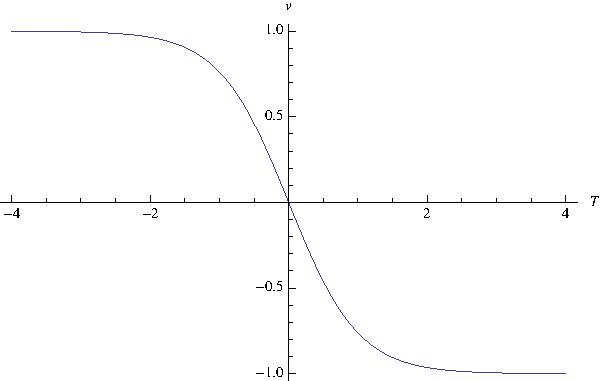
\includegraphics[width=0.6\textwidth]{tanh.pdf}
\caption{The x-axis is multiples of $\tau$ and the y axis is multiples of $v_{t}$}
\label{tanh}
\end{figure}

\section{Problem 5. Drag forces and horizontal motion.}

a.) This problem asks you to do the same thing as in problem 4 but to look at the horizontal component of the velocity. Here the important thing to remember is that the constant acceleration (g) doesn't act on the object in the horizontal direction. Also, the drag force on an object moving horizontally has to act against the motion so it will be a negative force. Therefore, the equation looks like this: \\
\begin{eqnarray*}
\frac{dv}{dt} &=& -bv^{2}  
\end{eqnarray*} \\
Then solve the same as before: \\
\begin{eqnarray*}
\frac{dv}{v^{2}} &=& -bdt \\
\int^{v_{0}}_{v}(v')^{-2}\,dv' &=& -b\int^{t}_{0}\,dt' =-b(t-0) \\
-(v')^{-1}|^{v}_{v_{0}} &=& -bt \\
(1/v - 1/v_{0}) &=& bt \\
1/v &=& bt +1/v_{0} \\
v &=& \frac{1}{bt + 1/v_{0}} \\ 
v_{x}(t) &=& \frac{v_{0}}{v_{0}bt + 1} 
\end{eqnarray*}  \\
This is a good point to check limits on the equation to see if it makes sense. First, we know that at time 0 the velocity should be the initial velocity and if you plug that in you can see that is indeed true. Second, as t approaches infinity the velocity should approach 0 and by taking the limit you see that is true also. Therefore, our solution makes physical sense. \\ \\
Find the time where v reaches half it's initial value, which is when $v_{x}/v_{0}=1/2$: \\ 
\begin{eqnarray*} 
v_{x}/v_{0} = 1/2 &=& \frac{1}{v_{0}bt+1} \\
(1/2)(v_{0}bt+1) &=& 1 \\
(1/2)v_{0}bt &=& 1/2 \\
t &=& \frac{1}{v_{0}b} 
\end{eqnarray*} \\
1/b has units of distance so it sets the characteristic distance for the problem. It is the distance over which the velocity decreases in the sense that how big or small 1/b is determines how fast the velocity decreases and the distance over which that decrease happens. This can be seen explicitly in the time it takes for the velocity to reach half its value. This time is proportional to 1/b meaning that the bigger 1/b is the longer it takes to reach half its velocity. Thus, 1/b sets the distance scale. \\ \\
b.) Now we need to calculate the fractional decrease of the baseball's velocity  $v/v_{0}$, but first we need to figure out a way to deduce the time for the given distance. Brian speaks of an ideal time which is from the ideal relationship of distance, velocity, and time without drag. \\ 
\begin{eqnarray*}
d &=& v_{0}t \\
t_{ideal} &=& d/v_{0} = 16 m/45 m/s = 0.36 s 
\end{eqnarray*} \\
Then plug this into the velocity equation from part a, but remember to make it the fractional velocity by dividing both sides by the initial velocity: \\ 
\begin{eqnarray*}
v_{x}(t)/v_{0} &=& \frac{1}{v_{0}bt_{ideal}+1} \\
v_{x}(t)/v_{0} &=& \frac{1}{(45m/s)(2x10^{-3}m^{-1})(0.36)s+1} = \frac{1}{1.03} \\
v_{x}(t)/v_{0} &=& 0.97 
\end{eqnarray*} \\ 
c.) Now we need to integrate the velocity equation from part a to get the horizontal position as a function of time. First turn $v_{x}(t) = \frac{dx}{dt}$ and group terms of x and t:
\\
\begin{eqnarray*}
v_{x}(t) &=& \frac{dx}{dt} = \frac{v_{0}}{v_{0}bt+1} \\ 
dx &=& \frac{v_{0}dt}{v_{0}bt+1} \\
\int^{x}_{0}\,dx' &=& \int^{t}_{0}\frac{v_{0}}{v_{0}bt'+1}\,dt' \\
u &=& v_{0}bt'+1 \\
du &=& v_{0}bdt', dt' = \frac{1}{v_{0}b}du \\
x &=& \int^{t}_{0}\frac{v_{0}}{v_{0}bu}\,du \\
x &=& (1/b)\ln(u)|^{t}_{0} \\
x &=& (1/b)\ln(v_{0}bt'+1)|^{t}_{0} \\
x &=& (1/b)\ln(\frac{v_{0}bt+1}{0+1}) = (1/b)\ln(v_{0}bt+1) \\
x(t) &=& (1/b) \ln(v_{0}bt+1) 
\end{eqnarray*} \\
d.) Now do a Taylor expansion on the horizontal distribution  around $t=0$, which will be useful for part d and e. \\
\begin{eqnarray*}
x(t)  &=& (1/b)\ln(v_{0}b(0)+1) +(1/1!)((1/b)\frac{v_{0}b}{v_{0}b(0)+1})(t-0) + (1/2!)((1/b)\frac{-v_{0^{2}}b^{2}}{(v_{0}b(0)+1)^{2}})(x-0)^{2} + ...\\
x(t) &=& (1/b) \ln(1) +(1/b)v_{0}bt -(1/2)(1/b)v_{0}^{2}b^{2}t^{2} +...\\
x(t) &=&  v_{0}t -(1/2)v_{0}^{2}bt^{2} + ... 
\end{eqnarray*} \\
Part d asks you to keep only the first non-zero term, which gives you: \\ 
\begin{eqnarray*} 
x(t) &\approx& v_{0}t 
\end{eqnarray*} \\
This is the same as the ``ideal'' solution you obtain when not using drag, which is the ``zeroth'' order correction. \\ \\
e.) The second non-zero term is the first order correction. \\ 
\begin{eqnarray*}
x(t) &\approx& v_{0}t -\frac{v_{0}^{2}bt^{2}}{2} 
\end{eqnarray*}  \\
f.) Calculate the ratio to get a rough estimate of the error on the approximation as done in problem 1. \\ 
\begin{eqnarray*}
err &\approx& \frac{v_{0}^{2}bt^{2}}{2v_{0}t} = \frac{v_{0}bt}{2} 
\end{eqnarray*} \\
Now plug in the ideal time from part b. \\ 
\begin{eqnarray*}
err &\approx& \frac{(45m/s)(0.002m^{-1})(0.36s)}{2} = 0.016 
\end{eqnarray*} \\
This means the error is about 1.6 percent which is relatively small, indicating this ideal time is a good approximation. \\ \\
g.) Calculate the time using the equation with the second term in the expansion from part e. \\ 
\begin{eqnarray*}
x(t) &\approx&  v_{0}t -\frac{v_{0}^{2}bt^{2}}{2} \\
16m &\approx& (45m/s)t - \frac{(45m/s)^{2}(0.002m^{-1})t^{2}}{2} \\
2.025t^{2} - 45t +16 &=& 0 \\
t &\approx& \frac{45±\sqrt{(45)^{2}-4(2.025)(16)}}{2(2.025)} = \frac{45±\sqrt{2025-129.9}}{4.05} \\
t&\approx& \frac{45±43.5}{4.05} = 21.9, 0.37 s 
\end{eqnarray*} \\
Note that we solved a quadratic equation and it had 2 roots. In physics usually only one root is actually a physical solution so make sure when solving quadratic equations to figure out which root makes physical sense and use that one. Here the 0.37 s is the physical solution since it is close to the ideal time and the other time is way off (not physical). \\ 
\begin{eqnarray*}
t_{1st} &\approx& 0.37 s 
\end{eqnarray*} \\ 
Now evaluate the fraction change of this time and the ideal time: \\ 
\begin{eqnarray*}
\frac{t_{1st}-t_{ideal}}{t_{ideal}} &=& 0.023 
\end{eqnarray*} \\
They differ by 2.3 percent. \\ \\
h.) Now the problem asks you to calculate the actual time using the horizontal position equation from part c. \\ 
\begin{eqnarray*} 
x(t) &=& (1/b) \ln(v_{0}bt+1) \\
16m &=& \frac{1}{0.002m^{-1}}\ln((45m/s)(0.002m^{-1})t+1) \\
0.032 &=&  \ln(0.09s^{-1}t+1) \\
0.09s^{-1}t+1 &=& e^{0.032} \\
0.09s^{-1}t &=& 1.033 - 1 \\
t &=& 0.033/0.09 = 0.367s
\end{eqnarray*} \\
This is very close to the ideal time and the first order correction to the time obtained in the previous parts of this problem. The fraction differences are: \\ 
\begin{eqnarray*}
\frac{t_{actual}-t_{ideal}}{t_{actual}} &=& 0.019 \\
\frac{t_{actual}-t_{1st}}{t_{actual}} &=& 0.0081 
\end{eqnarray*} \\
They are both small indicating that this ideal and 1st order approximation of the time is a good way to get the time. The 1st order is a better approximation though. This is something to keep in mind when you have more complicated equations where you can't analytically solve for the values that you want. In these cases you will want to use approximations like this to get to a solution and it is good to know how accurate these approximations are before you use them blindly. \\  \\

%% Problem 6. Kleppner and Kolenkow problem 1.21 \\ \\
%% A boy stands at the peak of a hill which slopes downward uniformly at an angle $\phi$. At what angle $\theta$ from the horizontal should he throw a rock so that is has the greatest range. \\ \\
%% We will need to calculate the range (R) and then take the derivative with respect to $\theta$ to maximize it. First lets find the kinematic equations: \\ 
%% \begin{eqnarray*}
%% x &=& x_{0} + v_{x0}t \\
%% v_{x0} &=& v_{0}\cos{\theta}, x_{0}=0 \\
%% x &=& v_{0}\cos{\theta}t \\
%% y &=& y_{0} +v_{y0}t - \frac{gt^{2}}{2} \\
%% v_{y0} &=& v_{0}\sin{\theta}, y_{0}=0 
%% \end{eqnarray*} \\
%% Then we need to deal with the extra amount $\phi$. This amount will be in a right triangle with the final range and final y. \\ 
%% \begin{eqnarray*} 
%% \tan{\phi} &=& -y_{f}/R 
%% \end{eqnarray*} \\
%% We want to find the time when $y=y_{f}$ so we can find $x=R$ at that point. \\ 
%% \begin{eqnarray*}
%% y_{f} &=& v_{0}\sin{\theta}t-\frac{gt^{2}}{2} \\
%% R &=& v_{0}\cos{\theta}t 
%% \end{eqnarray*} \\
%% The easiest time to solve for is in the range equation so find the time to get to the range and then plug it in to the y equation to get $y_{f}$. \\ 
%% \begin{eqnarray*}
%% t &=& \frac{R}{v_{0}\cos{\theta}} \\
%% y_{f} &=& \frac{Rv_{0}\sin{\theta}}{v_{0}\cos{\theta}} - \frac{gR^{2}}{2v_{0}^{2}cos^{2}(\theta)} \\
%% y_{f} &=& R\tan{\theta} - \frac{gR^{2}}{2v_{0}^{2}cos^{2}(\theta)} 
%% \end{eqnarray*} \\
%% Then plug in the equation for the final y in terms of R and $\phi$. \\
%% \begin{eqnarray*} 
%% -R\tan{\phi} &=& R\tan{\theta} -\frac{gR^{2}}{2v_{0}^{2}cos^{2}(\theta)} 
%% \end{eqnarray*} \\
%% Now solve for R and take the derivative with respect to $\theta$ and set it equal to 0 to maximize the range. The range will look very complicated at first, but then with some careful trig identities it can be simplified and the $\theta$ to maximize R can be found. \\ 
%% \begin{eqnarray*}
%% R &=& \frac{2v_{0}^{2}cos^{2}(\theta)}{g}(\tan{\theta}+\tan{\phi}) \\
%% \frac{dR}{d\theta} &=& \frac{2v_{0}^{2}}{g}(2\cos{\theta}(-\sin{\theta})(\tan{\theta}+\tan{\phi})+cos^{2}(\theta)(sec^{2}(\theta)))  = 0\\
%% 0 &=& (2\cos{\theta}(-\sin{\theta})(\tan{\theta}+\tan{\phi})+cos^{2}(\theta)(sec^{2}(\theta))) \\
%% 0 &=& -2sin^{2}(\theta)-2\cos{\theta}\sin{\theta}\tan{\phi}+1 \\
%% \cos{\theta}\sin{\theta} &=& (1/2)sin(2\theta) \mbox{ (trig identity)} \\
%% 0 &=& -2sin^{2}(\theta)-sin(2\theta)\tan{\phi}+1 \\
%% sin^{2}(\theta) &=& (1/2)(1-cos(2\theta)) \mbox{(half-angle formula)} \\
%% 0 &=& -1+cos(2\theta) -sin(2\theta)\tan{\phi} +1 \\
%% cos(2\theta) &=& sin(2\theta)\tan{\phi} \\
%% tan(2\theta) &=& \cot{\phi} \\
%% \theta &=& (1/2)tan^{-1}(\cot{\phi}) 
%% \end{eqnarray*} \\
%% Check the answer clue given in the book: \\ 
%% \begin{eqnarray*}
%% \phi &=& 60\degree \\
%% \theta &= &(1/2)tan^{-1}(\cot{\phi})=(1/2)tan^{-1}(1/\sqrt(3)) = \pi/6 = 15\degree 
%% \end{eqnarray*}  \\
%% which is what the book had. Try 2 more: \\ 
%% \begin{eqnarray*}
%% \phi &=& 45\degree \\
%% \theta &=& (1/2)tan^{-1}(1) = 45/2 = 22.5\degree \\
%% \phi &=& 0\degree \\
%% \theta &=& (1/2)tan^{-1}(\infty) = 90/2 = 45\degree 
%% \end{eqnarray*} \\
%% The last one is on flat ground. We can figure out geometrically that the angle has to be 45 degrees to maximize the range. This is a good check on this solution. \\ 

\end{document}












 





